\documentclass[12pt, preprint]{aastex}
\usepackage{bm}
\usepackage{amsmath}
\usepackage{booktabs}


\newcommand{\setof}[1]{\left\{{#1}\right\}}
\newcommand{\given}{\,|\,}
\newcommand{\dd}{\mathrm{d}}
\newcommand{\catalog}{\bm{Q}}
\newcommand{\pars}{\bm{\theta}}
\newcommand{\amin}{\ifmmode {^{\prime}\ }\else$^{\prime}$\fi}
\newcommand{\asec}{\ifmmode {^{\prime\prime}}\else$^{\prime\prime}$\fi}
\newcommand{\bs}[1]{\boldsymbol{#1}}

\newcommand{\Msun}{\ifmmode {M_{\odot}}\else${M_{\odot}}$\fi}
\newcommand{\Porb}{\ifmmode {P_{\rm orb}}\else${P_{\rm orb}}$\fi}
\newcommand{\sse}{{\tt SSE}}

\begin{document}

\title{Binary population synthesis with MCMC: \\ High-mass X-ray binaries and nearby star forming regions}
%\title{Modeling the X-Ray Populations of the SMC}
\author{some combination of JJA, AZ, TF, and others}
\date{NOT READY}

\begin{abstract}
Population models typically require a large number of simulation realizations, a computationally expensive endeavor, to generate statistically robust results. Employing Monte Carlo importance sampling, traditional population synthesis offers a substantial improvement over brute force, grid-based studies. However for certain problems, even population synthesis is limited by computational expense. We describe a novel approach which treats the initial binary parameters as model parameters, and uses a Markov Chain Monte Carlo technique to explore the valid region of parameter space. In addition to being substantially more efficient than traditional population synthesis methods, this approach has the fit to observational constraints built-in. Our technique is derived for correlating high mass X-ray binaries with star formation histories in the SMC, however this method can be flexibly adapted to other stellar populations. We test our method by successfully recovering input parameters for two synthetic binaries. We then apply our model to one particular system in the SMC, J0045$-$7319. Finally, we discuss future directions for this method. In the era of gravitational wave astronomy, efficient methods are needed to derive evolutionary histories for individual binary systems.
\end{abstract}





\section{Introduction}


The space-based X-ray observatory {\it Chandra} has revolutionized our understanding of X-ray luminous objects. Its unprecedented angular precision and collecting area allows it to identify dozens of resolved sources in nearby galaxies (references). Studies of individual objects have yielded a deeper insight into the physical processes forming the bulk of individually identified sources, low and high mass X-ray binaries, as well as a rare, but important subset, the ultra-luminous X-ray sources (references). High mass X-ray binaries (HMXB), in particular, are formed from the accretion of an early-type star onto either a neutron star or black hole (van den Heuvel?). Their relatively short lifetimes require that these systems cannot travel far away from their birth site, and indeed observations show that many of luminous X-ray sources are near star forming regions \citep{zezas02, kaaret04}. 

The nearby Small and Large Magellanic Clouds have the best studied extragalactic X-ray populations. Long term X-ray campaigns with {\it Chandra} have identified every X-ray emitting object with $L_x < 10^{32}$ erg s$^{-1}$ in the SMC, and ongoing observations of the somewhat larger LMC are approaching this degree of sensitivity (Zezas, Laycock et al.). At the same time, infrared, optical, and ultraviolet imaging with {\it HST} provide detailed spatially resolved star formation histories of the SMC and LMC with angular resolutions as small as 12\amin\ by 12\amin\ regions (Harris \& Zaritsky). These star formation histories are precise, particularly so over the past 10$^8$ yr when HMXBs were formed.


So far, models comparing regions of past star formation and the observed population of HMXBs have focused on the distance a population of HMXBs are expected to travel as a function of time \citep{sepinsky05} and how the distance can affect binary characteristics such as orbital period and X-ray luminosity \citep{zuo10, zuo15}. These models all employ population synthesis techniques.


Population studies typically seek to compare the likelihood of individual models to fit some set of astrophysical objects. Previous analysis of binary star populations have primarily relied on population synthesis, in which one randomly generates, according to some predetermined initial distribution of parameters, a large number of stellar binaries. By including our best understanding of binary evolution, this population is then evolved until its present state, when one then takes a ``snapshot'' of the binaries to determine the resulting population at a given time. Binary population synthesis models are typically employed for a number of tasks, including model comparison (kick velocities), learning about individual systems (e.g., M82 X-2), and predictions for as-yet unseen populations (e.g. LIGO). 


Discussion of StarTrack, Biceps, SeBa, BSE, others. Include general method and results. Reference comparison paper? By comparing to observed samples, Ihm et al and Andrews et al 2015 used a quantitative Bayesian method for model selection.


Yet, population synthesis is not the only method to populations of stars, and for rare or short-lived evolutionary states, it is exceedingly poor; significant computational time is spent on regions of parameter space of no interest to the observed systems. For HMXBs, specifically, mass transfer and supernova kicks may merge or disrupt the majority of systems. Therefore, in many binary population synthesis studies, $10^6-10^7$ binaries are required to make statistically robust comparisons with observed populations. An alternative is wanting.


Bhadkamkar \& Ghosh (2012) presented an alternative to population synthesis for HMXBs in which they analytically transformed the initial binary conditions 


 Instead of treating the kick velocity as a three-dimensional distribution, they applied the maximum likelihood value to a binary, reducing the marginalization in Equation \ref{eq:bayes} to a three-dimensional integral (the two initial masses and binary separation). Using Jacobian transformations, these authors analytically represented the current state of HMXBs as transformations of the initial conditions of a binary; they could determine exactly which initial conditions produced HMXBs with specific $L_x$. Subsequent integration over the remaining two parameters provided an X-ray luminosity function. However, this method was wanting in two separate aspects. First, their treatment of the SN kick velocity is an approximation, since they do not apply a distribution of kick velocities. Second, their analysis did not include the evolution over time. 






%at to characterize the population of HMXBs at a given time. By comparing the observed population of HMXBs in the SMC to the simulation ``snapshot'' after 60 Myr (the most recent ''starburst'' in the SMC), one can estimate the accuracy of our understanding of binary evolution. In essence population synthesis is a Monte Carlo numerical solution to the integral for the observed HMXBs:

In this work, we model the formation of HMXBs in a novel way using a Markov Chain Monte Carlo technique which naturally focuses computational power is on the region of parameter space relevant of interest. This method is versatile and substantially more efficient than comparable population synthesis methods, however care must be taken to properly normalize this prior distributions. {\bf More description of the method. By correlating the star formation histories to the present position of HMXBs, we can constrain the evolution of individual binaries, breaking degeneracies in their formation.} 





In Section \ref{sec:stats_population} we describe our statistical method for producing a synthetic population of HMXBs, comparing it with traditional population synthesis, and providing the relevant prior and posterior distributions. In Section \ref{sec:stats_individual} we extend our method to derive the constraints on the initial binary parameters that formed specific systems and provide these updated specific prior and posterior distributions. We provide the results for our model when run to produce a population of HMXBs in the SMC in Section \ref{sec:results_population}. In Section \ref{sec:results_individual} we produce our results for individual systems, first running two synthetic test binaries, then applying our model to the SMC binary PSR J0049$-$7319. We place our method in the broader context of binary population studies, providing some future directions in Section \ref{sec:discussion}. Finally, we provide some conclusions in Section \ref{sec:conclusions}.







\begin{comment}

We augment the problem to nine dimensions, adding the position and birth time as components of $\vec{x}_i$. Because of both its well characterized HMXB population and its precise star formation history, the SMC is an excellent testbed for this method. We apply our 9-parameter model to each HMXBs in the sample. Our results provide important constraints on both the binaries forming of each of these systems and the HMXB population of the SMC as a whole.

%NGC 55 is a relatively transparent, edge-on, nearby galaxy. Using the {\it Hubble Space Telescope}, and other optical telescopes, we have been able to identify a near-complete sample of star forming regions. For each region, multi-band photometry provides an estimate of the star formation history. 


%simulate the expected number, position, and characteristics of the X-ray binary population, given our sample of star forming regions, as well as the star formation history of the overall galaxy. We then apply a Bayesian method to generate a likelihood function comparing the resulting distribution with the observed X-ray sample.


\end{comment}



\section{Statistical Method: HMXB Population} \label{sec:stats_population}

% Traditional population synthesis
The goal of population synthesis is to randomly produce a set of binaries, $\{x_{\rm HMXB}\}$.\footnote{We focus on HMXBs, but the discussion can be generalized to any binary population.} Since we do not {\it a priori} know the distribution of HMXBs from first principles, traditional binary population synthesis solves this problem by making random draws from $\vec{x}_i$, the initial binary parameters:
\begin{equation}
\vec{x}_i \sim P(\vec{x}_i).
\end{equation}
To first order, HMXBs can be determined uniquely by the binary's initial masses, $M_{1,i}$ and $M_{2,i}$, its separation, $a_i$, and eccentricity $e_i$, and the kick velocity it received after the primary collapsed to form a NS or BH, $\vec{v}_k$. For the problem at hand, we also include the binary's birth position, $\alpha_i$ and $\delta_i$, and its birth time, $t_i$, for a total of ten parameters:
\begin{equation}
\vec{x}_i \equiv ( M_{1,i}, M_{2,i}, a_i, e_i, \vec{v}_k, \alpha_i, \delta_i, t_i ). \label{eq:x_i}
\end{equation}


Using a binary evolution code, these initial binaries are then evolved from $\vec{x}_i$ into its current state, represented by $\vec{x}_f$:
\begin{equation}
\vec{x}_f = f(\vec{x}_i). \label{eq:xf_xi}
\end{equation}
If the evolved binary forms an HMXB, it is kept, and if not, the randomly generated $\vec{x}_i$ is thrown away. This can be mathematically represented by a function $P(x_{\rm HMXB} \given \vec{x}_i)$ which is either unity or zero depending on whether $\vec{x}_f$ is a HMXB:
\begin{equation}
P(x_{\rm HMXB} | \vec{x}_i, M) = 
\begin{cases}
1, & \vec{x}_f \in x_{\rm HMXB} \\
0, & \vec{x}_f\ {\rm else}
\end{cases}
\end{equation}
Distributions of the components of $\vec{x}_f$ (such as the HMXB spatial distribution, X-ray luminosity function, orbital period distribution, etc.) can then provide model predictions for populations of HMXBs or comparisons to observations.




For binary populations involving neutron stars (NS) and black holes (BH), traditional population synthesis may be an inefficient tool; mass transfer and supernova kicks may merge or disrupt the majority of systems before they evolve into objects of interest ($P(x_{\rm HMXB} \given \vec{x}_i) = 0$ for many or even most of the randomly drawn $\vec{x}_i$). Such binaries are discarded. In many binary population synthesis studies, $10^6-10^7$ binaries are required to make statistically robust comparisons with observed populations.






% MCMC population synthesis
Instead of random draws of $\vec{x}_i$, we allow for the components of $\vec{x}_i$ to become model parameters. In this formulation $P(\vec{x}_i)$ is the prior probability on the model parameters, and $P(x_{\rm HMXB} \given \vec{x}_i)$ is the likelihood of producing an HMXB from a given $\vec{x}_i$. 
%(which is, again either unity or zero depending on whether $\vec{x}_i$ produces an HMXB). 
%This method draws samples of $\vec{x}_i$ based on the combined posterior probability $P(x_{\rm HMXB} \given \vec{x}_i) P(\vec{x}_i)$. 


In an MCMC implementation, a ``walker'' moves around the $\vec{x}_i$ parameter space: the posterior probability of the current $\vec{x}_i$ is calculated, a new trial $\vec{x}_i$ is randomly selected, the posterior probability of the new position is compared to that of the current position, and depending on the posterior probability ratio, the new $\vec{x}_i$ is either selected and added to the chain or rejected and the current position is kept for another step. A record of all the walker's past positions are stored in the chain. Samples from this chain comprise the synthetic population analogous to the population generated by traditional population synthesis.\footnote{Since the current walker position will necessarily be closely related to the previous step, the posterior samples will be correlated with some characteristic length. The correlation length needs to be calculated a posteriori, and only one sample per one correlation length can be considered independent.}


If implemented correctly, samples produced by this MCMC method will produce the same distribution of compact objects for identical $P(\vec{x}_i)$ and $P(x_{\rm HMXB} \given \vec{x}_i)$; for an infinite number of samples, the two distributions will be identical. The choice between traditional, importance-sampling population synthesis or the MCMC implementation described here should depend on formation efficiency of the binaries of interest. For high formation efficiencies, traditional methods are preferred. However, for HMXBs two separate effects make MCMC the preferred choice: most high mass binaries never become HMXBs and those that do are only X-ray emitting for a short portion of their lifetime.


Correct implementation requires careful attention to the prior distributions on $\vec{x}_i$, particularly normalization, and an efficient method to calculate $P(x_{\rm HMXB} \given \vec{x}_i)$. We describe, specifically, how we calculate the prior probabilities in Section \ref{sec:priors} and our single and binary evolution prescriptions in Sections \ref{sec:single_star} and \ref{sec:binary_evolve}, respectively.




% Priors
\subsection{Prior Probabilities: $P(M_{1,i}, M_{2,i,} a_i, e_i, \vec{v}_k, \alpha_i, \delta_i, t_i)$} \label{sec:priors}

Our model includes ten parameters. These are not necessarily independent of each other, however the prior probability can be factored into several parts:
\begin{eqnarray}
P(\vec{x}_i) &=& P(M_{1,i}) P(M_{2,i}\given M_{1,i}) P(a_i) \nonumber \\
 & & \qquad  \times\ P(e_i) P(\vec{v}_k \given M_{1,i}) P(\alpha_i, \delta_i, t_i)
\end{eqnarray}
We discuss each of these terms and the justification for their dependencies (where they exist) in turn below.

\subsubsection{Initial Binary Parameters}

As part of our model, we use standard distributions for the initial parameters of the binary. The initial primary mass follows a power law:
\begin{equation}
P(M_{1,i}) = C_m M_{1,i}^{\alpha},
\end{equation}
where $C_m$ is a normalization constant dependent upon the limits of the distribution ($M_{1,max}$ and $M_{1,min}$) and $\alpha$:
\begin{equation}
C_m = \frac{\alpha + 1}{M_{1,max}^{\alpha+1} - M_{1,min}^{\alpha+1}}.
\end{equation}
We choose 8 and 30 \Msun\ as the lower and upper mass limits that produce a NS. HMXBs formed with BH accretors are ignored. In practice, since the distribution strongly preferences lower mass stars, our results are relatively independent of the upper mass limit. We choose a Salpeter power law, such that $\alpha = -2.35$. Therefore $C$ can be determined:

We choose a prior on the secondary mass based on a flat mass ratio distribution which has a subtle effect that the prior on the secondary is dependent on the primary. The minimum mass ratio is 0.3, set by the limit for stable, thermal-timescale mass transfer, and the maximum mass ratio is unity. This can be shown to lead to a prior probability:
\begin{equation}
P(M_{2,i} \given M_{1,i}) = \frac{1}{0.7 M_{1,i}}.
\end{equation}

We choose a prior on the initial orbital separation of the binary that scales with $a^{-1}$:
\begin{equation}
P(a) = \frac{\log a_{max} - \log a_{min}}{a}
\end{equation}

Finally, we choose an Ambartsumian initial eccentricity distribution \citep{ambartsumian37, duquennoy91}:
\begin{equation}
P(e) = e^2.
\end{equation}


\subsubsection{SN Kick Parameters}

The SN kick velocity, $\vec{v}_k$, is composed of three parameters, which we model as a velocity ($v_k$) and two angles ($\theta_k, \phi_k$). In our model, we assume that $v_k$ follows a double Maxwellian distribution: one distribution for Fe-core collapse SN \citep[with a dispersion of 265 km s$^{-1}$][]{hobbs05}, and a separate Maxwellian distribution for electron-capture SN. $v_k$ therefore depends on $M_{1,i}$. We can therefore express the normalized probability of $v_k$ as:
\begin{equation}
P(v_k \given M_{1,i}) = \sqrt{\frac{2}{\pi}} \frac{v_k^2} {\sigma^3} {\rm exp} \left[ -v_k^2 / 2 \sigma^2 \right], \label{eq:P_v_k}
\end{equation}
where:
\begin{equation}
\sigma = 
\begin{cases} 
      50\ {\rm km/s}, & 8 < M_{1,i}/\Msun < 12: {\rm ECS}\\
     265\ {\rm km/s}, & 12 < M_{1,i}/\Msun: {\rm Fe-core\ SN}.
   \end{cases}
\end{equation}


Since the kick distribution is assumed to be isotropic, normalized probabilities for the kick polar, $\theta_k$, and azimuthal, $\phi_k$, angles are straightforward:
\begin{eqnarray}
P(\theta_k) &=& \sin \theta_k \in [0, \pi] \label{eq:P_theta_k} \\
P(\phi_k) &=& \frac{1}{2 \pi} \in [0, 2\pi] . \label{eq:P_phi_k}
\end{eqnarray}



\subsubsection{Star Formation History}

The priors on $\alpha_i$, $\delta_i$, and $t_i$ depends on the local star formation history at that position and time. We use the star formation history maps from Harris \& Zaritsky. We only take into account their star formation at a metallicity of $Z=0.008$, the dominant metallicity at which stars have been formed in the SMC over the past 1 Gyr. Their star formation history maps cover the SMC with some 1300 separate regions with angular resolutions of either 12\amin\ or 24\amin\ on a side. Each region has a resolution of 0.2 dex from log $t$ ranging from 6.8 to 10.2 yr. We ignore uncertainties on the star formation histories, generating an interpolation function for each region. 

These histories provide ${\rm SFR}(\alpha_i, \delta_i, t_i)$, the rate that stars were formed at a specific location and time in the SMC. When including a normalization constant, this spatially dependent star formation rate is the prior on position and time:
\begin{equation}
P(\alpha_i, \delta_i, t_i) = \frac{1}{N_{\rm SMC}} {\rm SFR}(\alpha_i, \delta_i, t_i),
\end{equation}
where $N_{\rm SMC}$ is the number of stars with $Z=0.008$ produced throughout the lifetime of the SMC.



\begin{figure}[h!]
\begin{center}
\includegraphics[width=0.75\columnwidth]{../figures/SMC_SF_history.pdf}
\caption{The prior on both position of the binary's birth location and time depends on the star formation history, derived from Harris \& Zaritsky. We show samples of the star formation history at four different times spanning the range of typical HMXB lifetimes. These demonstrate the typical resolution of the spatially-resolved star formation history.}
\label{fig:prior_SFH}
\end{center}
\end{figure}




% SSE
\subsection{Single Star Evolution} \label{sec:single_star}

Our single stellar evolutionary model is based on the stellar evolution fitting formulae, \sse, by \citet{hurley00}. Instead of using function calls within our code to \sse, we pre-compute a series of \sse\ models ranging in initial mass from 1.0 to 40.0 \Msun, with a spacing of 0.01 \Msun. These models use default parameters with a metallicity of 0.008 to match that of recent star formation in the SMC.

From the evolutionary history from \sse\ computed for each star (typically 200-500 time steps each), we use {\tt scipy}'s {\tt interp1d} routine to generate a linear interpolations across evolutionary stages for these stars. We interpolate as a function of time the key quantities: radius, mass, and mass loss rate. We then combine each of these {\tt interp1d} objects into an array. For any arbitrary mass star, to obtain quantities of interest, we round down to the next lowest mass interpolation. For a given input time, we can then obtain whatever fundamental quantity we are interested in. This method allows for fast calculation of fundamental properties of a star at an input age, while providing a sufficiently smooth transition over both mass and time.

Additionally, these models provide the minimum and maximum mass that produces a NS, core mass as a function of initial mass, maximum radius, stellar lifetime and H burning lifetime. For each of these, we create 1D interpolations as a function of initial mass.



% Binary evolution
\subsection{Binary Evolution} \label{sec:binary_evolve}

There are three major stages that we include in our binary evolution prescriptions. First, the more massive primary evolves first off the main sequence, leading to stable, thermal-timescale mass transfer onto the secondary. After the primary has completed its evolution it core-collapses, forming a NS. The system suffers effectively instantaneous mass loss and a natal kick, both of which act to profoundly affect the binary's orbit. Finally, the system begins to emit in X-rays once the NS accretes from the secondary's stellar wind. Since the companion's mass and mass loss rate change as the system evolves, these are both, in general, a function of time. We discuss each of these stages below.


% Thermal timescale mass transfer
\subsubsection{The First Mass Transfer Phase} \label{sec:trans_MT}

Once the first star evolves past its main sequence onto the giant branch, it begins overfilling its Roche lobe. We select only those systems that will undergo stable mass accretion, which can be determined by comparing the thermal time of the secondary with the mass accretion time. We discuss this further in Section \ref{sec:priors}. This comparison determines whether the transferring matter can lose its entropy fast enough to become incorporated with the companion star, or whether it forms a common envelope. We assume that the system instantaneously circularizes at the pericenter separation: $a_i (1-e_i)$. The post mass transfer primary becomes the primary core mass ($M_{1,c}$), while the secondary incorporates the primary's lost envelope. 
\begin{eqnarray} 
M_1' &=& M_{1,c} \\
M_2' &=& M_2 + M_1 - M_{1,c},
\end{eqnarray}
which assumes conservative mass transfer. The post-mass transfer orbital separation is:
\begin{equation}
a_{\rm MT} = a_i (1-e_i) \left[ \frac{M_1 M_2}{M_1' M_2'} \right]^2.
\end{equation}
$M_{1,c}$ is determined by the interpolations between \sse\ models described in Section \ref{sec:single_star}.


There is a subtle but important complication here. From the first mass transfer phase, the secondary gained a significant amount of hydrogen, which, depending on the initial stellar parameters, could more than double its mass. Clearly the stellar lifetimes will be affected. The first mass transfer phase will occur at roughly the helium ignition time for a star of mass $M_1$, $t_{\rm He} (M_1)$. If we assume that stars burn hydrogen at a constant rate throughout their main sequence, the hydrogen mass of the secondary at this point will be:
\begin{equation}
M_{\rm He,2} = \frac{t_{\rm He}(M_{1,i})}{t_{\rm He}(M_{2,i})} M_{\rm He,core}(M_{2,i}), \label{eq:M_He}
\end{equation}
where $M_{\rm He,core}(M_{2,i})$ is the helium core mass (at helium ignition) of a star with an initial mass of $M_{2,i}$. At this point, the secondary will accrete roughly pure hydrogen from the primary. Since this mass transfer occurs on a thermal timescale, it is effectively instantaneous compared to the stellar lifetime. The rejuvenated secondary star may have a substantially different mass ($M'_2$), but it is not beginning with a cosmological helium abundance. We can estimate its effective age ($t_{\rm eff}$) by comparing its helium mass from Equation \ref{eq:M_He} with $M_{\rm He,core}(M_2')$, multiplied by the helium ignition time:
\begin{equation}
t_{\rm eff} = \frac{M_{\rm He,2}}{M_{\rm He,core} (M_2') } t_{\rm He} (M_2'). \label{eq:t_eff_1}
\end{equation}
Finally, the total age of the system ($t_i$) is a conditional on our posterior probability. The secondary's effective age at the time of observation, $t_i$, is $t_{\rm eff,obs} = t_{\rm eff} + t_i - t_{\rm He}(M_{1,i})$, which can be expressed using Equations \ref{eq:M_He} and \ref{eq:t_eff_1}:
\begin{equation}
t_{\rm eff,obs} = \frac{M_{\rm He,core}(M_{2,i})}{M_{\rm He,core}(M_2')} \frac{t_{\rm He}(M_{1,i})}{t_{\rm He}(M_{2,i})} t_{\rm He}(M_2')
  + t_i - t_{\rm He}(M_{1,i}) \label{eq:t_eff_obs_full}
\end{equation}
Using this effective time in the interpolations, we can determine the adjusted mass, radius, and wind mass loss rate of the secondary using single stellar evolution models. 


\subsubsection{The Primary's Core Collapse} \label{sec:trans_SN}

We next calculate the post-SN orbital separation, $a_{\rm SN}$, systemic velocity, $v_{\rm sys}$, and eccentricity, $e_{\rm SN}$ based on the equations in Hills (1983) and Kalogera (1996). Energy conservation provides $a_{\rm SN}$:
\begin{equation}
a_{\rm SN} = \left[ \frac{2 }{a_{\rm MT}}  - \frac{v_1^2}{G(M_{\rm NS} + M_2')} \right]^{-1}. \label{eq:SN_A} \\
\end{equation}
where $v_1$ is the post-kick velocity of the primary (in the reference frame of an initially stationary secondary):
\begin{equation}
v_1^2 = 2v_k v_r \cos \theta + v_k^2 + v_r^2. \label{eq:v_1}
\end{equation}
Here, we have made the additional substitution:
\begin{equation}
v_r = \sqrt{\frac{G (M_1' + M_2')}{a_{\rm MT}}}. \label{eq:v_r}
\end{equation}
The systemic velocity is:
\begin{equation}
v_{\rm sys}^2 = \beta^2 v_k^2
   + v_r^2 \left( \alpha - \beta \right)^2
   + 2 \beta v_r v_k \cos \theta \left( \alpha - \beta \right)
    \label{eq:SN_v_sys}
\end{equation}
where we have included two substitutions:
\begin{eqnarray}
\alpha &=& \frac{M_1'}{M_1' + M_2'} \\
\beta &=& \frac{M_{\rm NS}}{M_{\rm NS} + M_2'}
\end{eqnarray}


The post-SN eccentricity is determined by angular momentum conservation:
\begin{equation}
1-e_{\rm SN}^2 = \frac{a_{\rm MT}^2}{a_{\rm SN}\ G (M_{\rm NS} + M_2')} \left[ v_k^2 \cos^2\theta + v_k^2 \sin^2 \theta \sin^2 \phi + 2 v_k v_r \cos \theta + v_r^2  \right]. \label{eq:SN_e}
\end{equation}
Systems with $0 \leq e < 1$ remain bound. We do not include tidal dissipation or circularization, but keep track of $e_{\rm SN}$ since it affects the X-ray luminosity calculation below.




\begin{comment}
The reverse mapping of this transformation, $H_{\rm SN}$ is analytic. We first make a substitution:
\begin{eqnarray}
X &=& \frac{\beta - \alpha}{\beta} v_r \nonumber \\
&=& -v_k \cos\theta \pm \sqrt{\frac{v_{\rm sys}^2}{\beta^2} - v_k^2 \sin^2\theta}, \label{eq:SN_X}
\end{eqnarray}
which we obtain by solving Equation \ref{eq:SN_v_sys} for $v_r$. Combining Equations \ref{eq:SN_A}, \ref{eq:v_1}, \ref{eq:v_r}, and \ref{eq:SN_X}, we obtain a quadratic equation for $M_1'$:
\begin{equation}
0 = C_1 M_1'^{2} + C_2 M'_1 + C_3, \label{eq:SN_M_1}
\end{equation}
where the constants, $C_i$, are equal to:
\begin{eqnarray}
C_1 &=& \frac{G(M_{\rm NS} + M'_2)}{A''} + v_k^2 + \frac{M_{\rm NS}^2}{M_2^{'2}}X^2 - 2 v_k \cos \theta \frac{M_{\rm NS}}{M'_2}X \\
C_2 &=& -2M_{\rm NS} \left[ \frac{G(M_{\rm NS} + M'_2)}{A''} + v_k^2 + \frac{M_{\rm NS}^2}{M_2^{'2}}X^2 + \left( 1 - \frac{M_{\rm NS}}{M'_2} \right) v_k \cos \theta X \right] \\
C_3 &=& \frac{G(M_{\rm NS} + M'_2)}{A''} M_{\rm NS}^2 + M_{\rm NS}^2 (v_k^2 + X^2) + 2v_k \cos \theta M_{\rm NS}^2 X - \frac{2(M_{\rm NS} + M'_2)}{M'_2} M_{\rm NS}^2X^2
\end{eqnarray}
Solving Equation \ref{eq:SN_M_1} now provides four separate values for $M_1'$, each of which has a corresponding $A'$ value:
\begin{equation}
A' = G (M_1' + M_2') \left(\frac{M_{\rm NS} - M_1'}{M_1' + M_2'} \right)^2 \left( \frac{M_2'}{M_{\rm NS}} \right)^2 \frac{1}{X^2}. \label{eq:SN_A1}
\end{equation}
Although there are four separate solutions for $M_1'$ and $A'$, three can be removed since we require that $v_r > 0$ and $M'_1 > M_{\rm NS}$. All four must be solved for since it is unknown which of the four solutions is the correct one {\it a priori}.



Derivatives of equations \ref{eq:SN_A} and \ref{eq:SN_v_sys} determine the Jacobian $J_{\rm SN}$. We provide the analytic form for $J_{\rm SN}$ in the Appendix. The probability of the post-SN parameters from the pre-SN parameters and the three kick parameters is:
\begin{equation}
P(M_{\rm NS}, M_2', A'') = P(M_1', M_2', A') J_{\rm SN}. \label{eq:P_SN}
\end{equation}
\end{comment}




\subsubsection{The X-ray Luminous Phase} \label{sec:trans_XRB}

{\bf REWRITE: This method can be used in the future to determine $L_x$, but currently incomplete.}

Once the secondary evolves onto the core helium burning phase, its luminosity increases, and the star emits a wind accreted by the primary NS. Determining the X-ray luminosity ($L_x$) from the accretion rate ($\dot{M}$) is straightforward: 
\begin{equation}
L_x = \frac{G M_{\rm NS} \dot{M}}{R_{\rm NS}}.
\end{equation}
Since the stellar wind is faster than the orbital velocity of the companion, the orbital separation, $a_{\rm XRB}$, is significantly greater than the Bondi radius of the NS. Under this assumptions, the fraction of the companion's wind that is accreted by the NS can be determined in a straightforward way:
\begin{equation}
\dot{M} = \left( \frac{G M_{\rm NS}}{V_w^2\ a_{\rm XRB}} \right)^2 \times \dot{M}_{\rm wind}. \label{eq:mdot}
\end{equation}
Unfortunately, $\dot{M}_{\rm wind}$ is not a simple function of the stellar mass. To solve this problem, we use the interpolation over $\dot{M}$ in time described in Section \ref{sec:single_star}. 

Equation \ref{eq:mdot} is dependent upon the fourth power of $V_w$, and must therefore be treated carefully. Based on studies of O and B star winds, Vink et al.\ determine that the terminal stellar wind velocity scales with the escape velocity by a factor, $\beta$, of order unity. Specifically, we use:
\begin{equation}
V_w = \sqrt{\frac{2 \beta G M}{R^2}},
\end{equation}
where $\beta$ is linearly interpolated between 1.4 for 120 \Msun\ stars and 0.5 for 7 \Msun\ stars. Again, we use the \sse\ interpolation outputs to obtain estimates of $M$ and $R$ as a function of initial mass and time.

These binary routines completely evolve a binary from a set of initial conditions, $\vec{x}_i$, to its current state. If the system has evolved into a HMXB, then $P(\vec{x}_f \given \vec{x}_i)$ is unity, otherwise it is zero.













% Individual HMXBs
\section{Statistical Method: Individual HMXBs} \label{sec:stats_individual}

If we would like to quantitatively compare a model to a set of observed systems, we need to adapt our method. We may be interested in either deriving the initial binary conditions that could have produced the observed systems, $P(\vec{x}_i \given x_{\rm HMXB})$, or determining binary parameters that have not yet been observed, $P(\vec{x}_f \given x_{\rm HMXB})$. From Equation \ref{eq:xf_xi}, binary evolution relates $\vec{x}_f$ to $\vec{x}_i$, therefore these two problems are closely related. 


%We may be interested in either the probability of a model given the set of observed systems, $P(M \given \{x_{\rm HMXB}\})$, or deriving the initial binary conditions that could have produced the observed systems, $P(\{\vec{x}_i\} \given \{x_{\rm HMXB}\})$.  


We cannot directly calculate $P(\vec{x}_i \given x_{\rm HMXB})$. Instead, we can calculate $P(x_{\rm HMXB} \given \vec{x}_i)$, the probability that the set of initial binary parameters produces a system like the one observed. These two conditional probabilities can be linked using Bayes' theorem:
\begin{equation}
P(\vec{x}_i \given x_{\rm HMXB}) = \frac{P(x_{\rm HMXB} \given \vec{x}_i)\ P(\vec{x}_i)}{P(\vec{x}_{\rm HMXB})}, \label{eq:bayes}
\end{equation}
where $P(\vec{x}_i)$ is the prior probability on the initial binary parameters and $P(\vec{x}_{\rm HMXB})$ is a normalization constant. 

Traditional population synthesis takes a shotgun approach to calculating these probabilities, making random draws of $\vec{x}_{i,j}$ from $P(\vec{x}_i)$. After a large number of random draws of $\vec{x}_{i,j}$, the likelihood function selects only those systems that are consistent with the observed system. Results are then drawn from those systems with non-zero posterior probabilities. The likelihood function is more complex here than that used previously since it should include observational uncertainties, as well as system-specific data. We discuss in detail both the prior distribution and the likelihood function in Sections \ref{sec:priors_indiv} and \ref{sec:likelihood_indiv} below. Since only a small subset of the binaries that form HMXBs will be consistent with any particular observed system, the likelihood function is non-zero for only a small region of parameter space. Traditional population synthesis methods are extremely inefficient for this problem, and obtaining enough statistics such that the relevant region of initial parameter space is sufficiently explored is computationally expensive.




%\begin{equation}
%P(M \given \{x_{\rm HMXB}\}) = \frac{P(\{x_{\rm HMXB}\} \given M)\ P(M)}{P(\{x_{\rm HMXB}\})}, \label{eq:bayes}
%\end{equation}
%where $P(M)$ is the prior probability on the model, $P(\{x_{\rm HMXB}\})$ is the so-called evidence, and $P(\{x_{\rm HMXB}\} \given M)$ is the likelihood of the data given the model. Now, we marginalize over the set of possible initial binary conditions for each object, $\{\vec{x}_i\}$:
%\begin{eqnarray}
%P(\{x_{\rm HMXB}\} \given M) &=& \int \dd \{\vec{x}_i\}\ P( \{x_{\rm HMXB}\} \given \{\vec{x}_i\}, M )\ P(\{\vec{x}_i\} \given M) \nonumber \\
% &=& \int \dd \{\vec{x}_i\}\ \prod_{{\rm all}\ x_{\rm HMXB}} P( x_{\rm HMXB} \given \vec{x}_i, M )\ P(\vec{x}_i \given M) \nonumber \\
% &=& \prod_{{\rm all}\ x_{\rm HMXB}} \int \dd \vec{x}_i\ P( x_{\rm HMXB} \given \vec{x}_i, M )\ P(\vec{x}_i \given M)  \label{eq:P_x_marginalized}
%\end{eqnarray}
%where $P( x_{\rm HMXB} \given \vec{x}_i, M )$ is the likelihood function for each HMXB, and $P(\vec{x}_i \given M)$ is the prior on $\vec{x}_i$. We were able to move the product over all HMXBs outside the integral since each object is an unique sample, independent of the others.



%Traditional population synthesis provides a numerical solution to this multidimensional integral:
%\begin{equation}
%P(x_{\rm HMXB} \given M) \approx \frac{1}{N} \sum_{j \in N} P( x_{\rm HMXB} \given \vec{x}_{i,j}, M ), \label{eq:x_i_marginalize_sum}
%\end{equation}
%where $\vec{x}_{i,j}$ are drawn from the prior probabilities:
%\begin{equation}
%\vec{x}_{i,j} \sim P(\vec{x}_i \given M).
%\end{equation}


In our method, the prior probabilities and likelihood function are the same as for traditional population synthesis, however we treat $\vec{x}_i$ as a set of model parameters, reducing this to an optimization problem. Since the likelihood function is restricting, the efficiency of computation between the MCMC method described here and the traditional population synthesis method is substantial. Samples from the posterior distribution provide $P(\vec{x}_i \given x_{\rm HMXB})$, which can provide astrophysical implication about how individual systems formed.

%The method however makes a different approximation:
%\begin{equation}
%P(x_{\rm HMXB} \given M) \approx \frac{1}{N} \sum_{j \in N} P( x_{{\rm HMXB},j}),
%\end{equation}
%where $x_{{\rm HMXB},j}$ are samples drawn from the posterior probability:
%\begin{equation}
%x_{{\rm HMXB},j} \sim P( x_{\rm HMXB} \given \vec{x}_i, M ) P(\vec{x}_i \given M).
%\end{equation}











%In this method, every component of $\vec{x}_i$ is a model parameter. $P(\vec{x}_i \given M)$ is the prior probability on $\vec{x}$ and $P(D \given \vec{x}_f, M)\ P(\vec{x}_f \given \vec{x}_i, M)$ is the likelihood function. We cannot directly generate a large sample of $D_j$. Instead, MCMC provides an algorithm that probes the $\vec{x}_i$ parameter space incrementally to create a sample. For binary evolution, in which $P(D \given \vec{x}, M)$ has substantial structure, this form can be substantially more efficient, since substantially less computational time is spent evolving systems outside the parameter space region of interest. The cost of this method is additional overhead in the process, since the likelihood must be calculated at every step, for every $\vec{x}_i$, before the next $\vec{x}_i$ can be chosen.








We simulate individual HMXBs using the same model parameters as we use for a population, so $\vec{x}_i$ is determined by Equation \ref{eq:x_i}. However, HMXBs in the SMC and LMC may have well measured $P'_{\rm orb}$, $e'$, and $M'_2$ determined from identifying the observational counterpart to the X-ray source. Each of these measured quantities has some uncertainty associated with it. Furthermore, individual HMXBs have a specific location that we are trying to associate with nearby star forming regions. Therefore, the likelihood function in Equation \ref{eq:P_x_marginalized} is somewhat more complicated. We start by defining $D$ as:
\begin{equation}
D \equiv (\alpha, \delta, P'_{\rm orb}, e', M'_2). \label{eq:D}
\end{equation}
We use primed quantities to denote observed values that are, in general, different from the true, physical values $P'_{\rm orb}$, $e'$, and $M'_2$. We ignore uncertainties on the position.


To generate our likelihood function, we now marginalize over four parameters, the true orbital parameters, $P_{\rm orb}$ and $e$, the true (current) companion mass $M_2$, and the systemic velocity ($v_{\rm sys}$):
\begin{equation}
P(D \given \vec{x}_i, M) =  \int \dd P_{\rm orb}\ \dd e\ \dd M_2\ \dd v_{\rm sys}\ P( P_{\rm orb}, e, M_2, v_{\rm sys}, D \given \vec{x}_i, M).
\end{equation}
Based on independence, we express this integral into separate, tractable parts:
\begin{eqnarray}
P(D \given \vec{x}_i, M) &=&  \int \dd P_{\rm orb}\ \dd e\ \dd M_2\ \dd v_{\rm sys}\ P(P'_{\rm orb} \given P_{\rm orb}) \nonumber \\
	& & \qquad \times P(e' \given e)\ P(M'_2 \given M_2) \nonumber \\
	& & \qquad \times P(\alpha, \delta \given \alpha_i, \delta_i, t_i, M_{1,i}, v_{\rm sys}) \nonumber \\
	& & \qquad \times P(P_{\rm orb}, e, M_2, v_{\rm sys} \given M_{1,i}, M_{2,i}, a_i, e_i, \vec{v}_k, t_i). \label{eq:marginalized}
\end{eqnarray}
The two terms in the integrand, $P(P'_{\rm orb} \given P_{\rm orb})$ and $P(e' \given e)$, include the observational uncertainties on the binary's orbit. We model these with Gaussian uncertainties, but in principle, can account for any observationally-derived distribution. Similarly, $P(M'_2 \given M_2)$ accounts for the observational uncertainty on $M_2$. This term again can be approximated as a Gaussian distribution, but a more careful determination will include a comparison between the observed magnitudes in various filters and stellar models on a color-magnitude diagram. 

The fourth term in the integrand accounts for the fact that the system's birth place may, in general, be different from its observed position since the center of mass of a system received a kick during the primary's core collapse. We explicitly include dependencies on $v_{\rm sys}$, $t_i$, and $M_{1,i}$ since the distance travelled depends on both the system's velocity and time since the primary's supernova. We derive this term in Section \ref{sec:ra_dec} below. 

The last term of the integrand, which we discuss in Section \ref{sec:binary_evolve}, includes the binary evolution from its {\it ab initio} state to the $P_{\rm orb}$, $e$, $M_2$, and $v_{\rm sys}$ of the system today. In section \ref{sec:priors} we derive the prior distributions for each of our ten model parameters.



\subsection{Priors} \label{sec:priors_indiv}


\begin{figure}[h!]
\begin{center}
\includegraphics[width=0.55\columnwidth]{../figures/prior_SFH.pdf}
\caption{The prior on both position of the binary's birth location and time depends on the star formation history. Only the star formation history within the cone, the size and shape of which is set by the binary parameters, are taken into account. We show contours indicating regions of high (red) and low (blue) star formation for three different ages. Determining the prior on the star formation history involves integrating the star formation history throughout the cone.}
\label{fig:prior_SFH}
\end{center}
\end{figure}

Figure \ref{fig:prior_SFH} demonstrates how we determine the normalization constant. An object at a location $(\alpha, \delta)$ could have been formed only within a region (shown by the circle) that progressively increases for older birth times. Only stars formed within this cone contribute to the normalization constant; stars formed outside the cone could not have led to the observed system. The shape and size of the cone changes depending on the binary parameters (hence the conditional dependence on this term), therefore the prior needs to be recalculated for each set of model parameters. Because of the function calls, calculating this normalization constant is the most computationally expensive portion of this method. 

The normalization constant is determined by integrating over the specific star formation rate throughout the cone and setting the quantity to unity:
\begin{equation}
1 = C_{\rm SFH}\ \int_{t_{min}}^{t_{max}} \int_0^{2 \pi} \int_0^{\theta_c} \dd t_i\ \dd \phi\ \dd \theta\ {\rm SFR}(\theta, \phi, t_i). 
\end{equation}
We choose to calculate the integral using a Monte Carlo sampling technique. We draw $N$ random samples throughout the cone. The integral is the product of the average of the samples and the cone's volume:
\begin{equation}
\frac{1}{C_{\rm SFH}} \approx \frac{\pi \theta_C^2 (t_{max} - t_{min})}{3N} \sum_j {\rm SFR}(\theta_j, \phi_j, t_{i,j}),
\end{equation}
where $(\theta_j, \phi_j, t_{i,j})$ are random samples, evenly distributed around the cone's volume. Formally, an infinite number of samples is required for the approximation above to become an equality, however, we find that for typical systems, 512 samples is sufficient to accurately calculate $C_{\rm SFH}$.



 To obtain random samples of $\theta$ and $t$, we use inversion sampling, which involves obtaining random samples of the cumulative distribution function. The random values of $\theta$ and $t$ are the inversions of those samples:
 \begin{eqnarray}
\phi &\sim& U(0, 2\pi) \\
\theta &=& \sqrt{\frac{y}{C_{\theta}(t) \pi}}: y \sim U(0,1) \\
t &=& \left[ \frac{3y}{C_t \pi \left( \frac{v_{sys}}{D_{\rm SMC}} \right)^2} \right]^{1/3} + t(M_{1,i}): y \sim U(0,1)], 
\end{eqnarray}
where:
\begin{eqnarray}
C_{\theta} &=& \frac{1}{\pi \theta_c^2(t)} \\
C_t &=& \frac{ 3 \left( \frac{D_{\rm SMC}}{v_{sys}} \right)^2 }{ \pi \left( t_{max} - t_{min} \right)^3 }.
\end{eqnarray}
Since $C_{\theta}$ depends on the $t$, we must generate random samples in $t$ first. 






\subsection{Likelihood Function} \label{sec:likelihood_indiv}
%\subsubsection{Position Probability: $P( \alpha, \delta \given \alpha_i, \delta_i, t_i, M_{1,i}, v_{\rm sys} )$} \label{sec:ra_dec}

\subsection{Binary Parameter Likelihood}

Our method can adapt to any observations of individual stellar parameters.

For HMXBs, we use three separate observables: $M'_2, P_{\rm obs},$ and $e$.

Define Gaussian distributions for these three. 

\subsection{Position Likelihood}
The first term provides the probability that, given a system's birth time, position, systemic velocity, and initial primary mass, the system would be observed at its current position. Since HMXBs are generally short lived, this probability is non-zero for only a small region around any given HMXB's observed position. To solve the positional component of Equation \ref{eq:marginalized}, we first marginalize over $\omega$ the angle between the line of sight vector to the birth location and the systemic velocity vector:
\begin{equation}
P(\alpha, \delta \given \alpha_i, \delta_i, t_i, M_{1,i}, v_{\rm sys} ) = \int \dd \omega\ P(\alpha, \delta, \omega \given \alpha_i, \delta_i, t_i, M_{1,i}, v_{\rm sys} ). \label{eq:P_pos_1}
\end{equation}

\begin{figure}[h!]
\begin{center}
\includegraphics[width=0.95\columnwidth]{../figures/position_projected.pdf}
\caption{Our representation of the current position $(\alpha, \delta)$ in relation to its birth position $(\alpha_i, \delta_i)$. The distance the system traveled is $d$, which has a projected separation $s$. We express this transportation as a function of $\theta_{\rm proj}$ and position angle, $\phi$. Note, for typical systems $d << D_{\rm SMC}$.}
\label{fig:position_projection}
\end{center}
\end{figure}


We next perform a coordinate transform from the absolute positional coordinates $\alpha$ and $\delta$ to the angular separation, $\theta_{\rm proj}$, and the position angle, $\phi$, measured from the system's birth location. The determinant of the Jacobian matrix for this transformation is:
\begin{equation}
J_{\rm coor} = \left| \frac{\dd \alpha}{\dd \theta_{\rm proj}} \frac{\dd \delta}{\dd \phi} - \frac{\dd \alpha}{\dd \phi} \frac{\dd \delta}{\dd \theta_{\rm proj}} \right|.
\end{equation}
Equation \ref{eq:P_pos_1} now becomes:
\begin{eqnarray}
P(\alpha, \delta \given \alpha_i, \delta_i, t_i, M_{1,i}, v_{\rm sys} ) &=& \int \dd \omega\ P(\theta_{\rm proj}, \phi, \omega \given t_i, M_{1,i}, v_{\rm sys} ) J_{\rm coor}. \nonumber \\
&=& \int \dd \omega\ P(\theta_{\rm proj} \given \omega,  t_i, M_{1,i}, v_{\rm sys} )\ P(\phi)\ P(\omega)\ J_{\rm coor}, \label{eq:P_pos_2}
\end{eqnarray}
where we have separated terms based on independence; $\omega$ is a randomly chosen polar angle and $\phi$ is a randomly chosen azimuthal angle with normalized probabilities, respectively: 
\begin{eqnarray}
P(\omega) &=& \frac{\sin \omega} {2}, \in [0,\pi] \\
P(\phi) &=& \frac{1}{2 \pi}, \in [0, 2\pi].
\end{eqnarray}


The physical distance an HMXB travels is the product of $v_{\rm sys}$ and the time since the primary's core collapse:
\begin{equation}
d = v_{\rm sys} \left[t_i - t(M_{1,i}) \right],
\end{equation}
where $t(M_{1,i})$ is the lifetime of a star with a mass of $M_{1,i}$. We can only observe the projection of $d$ onto the sky, $s = d \sin \omega$. $s$ is approximated as the product of the distance to the SMC, $D_{\rm SMC}$ and $\theta_{\rm proj}$, which allows us to express $\theta_{\rm proj}$ in terms of model parameters:
\begin{equation}
\theta_{\rm proj} = \frac{v_{\rm sys} \left[ t_i - t(M_{1,i}) \right] \sin \omega}{D_{\rm SMC}}. \label{eq:theta_proj}
\end{equation}
The third term in the integrand in Equation \ref{eq:P_pos_2} is a delta function:
\begin{equation}
P(\theta_{\rm proj} \given \omega, t_i, M_{1,i}, v_{\rm sys}) = \delta \left[G(\omega)\right], \label{eq:P_theta_proj}
\end{equation}
where:
\begin{equation}
G(\omega) = \theta_{\rm proj} - \frac{v_{\rm sys} \left[t_i - t(M_{1,i}) \right] \sin \omega}{D_{\rm SMC}}.\end{equation}


With the delta function from Equation \ref{eq:P_theta_proj}, the integral in Equation \ref{eq:P_pos_2} can be reduced:
\begin{equation}
\int \dd \omega\ P(\phi) P(\omega) \delta \left[ G(\omega) \right]  J_{\rm coor}\  =\ \sum_i\ \frac{P(\omega_i^{\star}) P(\phi)  J_{\rm coor}}{ \left| \frac{ \dd G (\omega) }{\dd \omega} \right|_{\omega_i^*}},
\end{equation}
where $G(\omega)$ is the function inside the delta function in Equation \ref{eq:P_theta_proj} and the sum is over $\omega_i^*$, the $i$ roots of $G(\omega)$. There are two roots corresponding to whether the object is in front of or behind its birth location. This integral can now be evaluated analytically:
\begin{equation}
P(\alpha, \delta \given \alpha_i, \delta_i, t_i, M_{1,i}, v_{\rm sys} ) =
\begin{cases} 
      0, & \theta_{\rm proj} \geq \theta_C\\
     \frac{\tan \omega^*}{2 \pi \theta_C}  J_{\rm coor}, & \theta_{\rm proj} < \theta_C 
   \end{cases}
\end{equation}
where:
\begin{equation}
\omega^{\star} = \sin^{-1} \left[ \frac{\theta_{\rm proj}}{\theta_C} \right].
\end{equation}
and
\begin{equation}
\theta_C = \frac{v_{\rm sys} \left[ t_i - t(M_{1,i}) \right]}{D_{\rm SMC}} \label{eq:theta_c}
\end{equation}


\subsubsection{Binary Probability: $P(L_x, M_2, v_{\rm sys} \given M_{1,i}, M_{2,i}, a_i, e_i, \vec{v}_k, t_i)$}

Given a birth time and a particular initial binary parameters, this term provides the probability that a binary with a particular $L_x$, $M_2$, and $v_k$ will be formed. For HMXBs, determining this term relies on the evolution through three separate evolutionary transitions. 




\section{Results: Population of HMXBs} \label{sec:results_population}


\begin{figure}[h!]
\begin{center}
\includegraphics[width=0.95\columnwidth]{../figures/smc_population_corner.pdf}
\caption{ The covariances and 1D histograms of our posterior distribution that produces HMXBs in the SMC. Some of the posterior distributions closely reflect the priors probabilities, however others, such as $v_k$, $\theta_k$, and $t_b$, show substantial differences. The covariance between $\alpha_i$ and $\delta_i$ should closely follow the spatially resolved star formation rate over the posterior distribution of birth times. That the distribution is patchy indicates the walkers seem to have no trouble exploring the entire spatial parameter space.}
\label{fig:population_corner}
\end{center}
\end{figure}



\begin{figure}[h!]
\begin{center}
\includegraphics[width=0.55\columnwidth]{../figures/smc_population_HMXB_ra_dec.pdf}
\caption{ Colored regions indicate the star formation rate in the SMC 30 Myr ago, while contours show the posterior distribution of the system's birth position. The contours define a region substantially larger than the SMC, indicating that HMXBs can, indeed, move large distances away from the SMC while still in their X-ray luminous phase. Note, 1 degree is $\approx$ 1 kpc.}
\label{fig:population_ra_dec}
\end{center}
\end{figure}



To explore the parameter space based on the posterior probability in Equation \ref{eq:posterior_population} we opt for the MCMC code {\tt emcee} \citep{foreman-mackey13}. {\tt emcee} employs an affine-invariant ensemble sampler using multiple ``walkers" in concert\citep{goodman10}. Our model uses 80 walkers. We discuss in detail our method to initialize these walkers in the Appendix. For now, we only mention that, since a large portion of the parameter space has a zero probability, it must be ensured that the walkers are initialized in non-zero regions of parameter space. After initializing, we run {\tt emcee} for a ``burn-in" of 10,000 steps. We then run our simulation for 50,000 steps to gain sufficient statistics. We check the chains to make sure they have converged; we find autocorrelation lengths of $\sim$100 steps across model parameters, and an acceptance fraction of {\bf XXX}. 

Figure \ref{fig:population_corner} shows covariances between the posterior distribution of model parameters. That these covariances produce well defined regions for the majority of parameters is indicative that our model is able to explore effectively the relevant parameter space. 

Distributions over $M_1$ and $M_2$ strongly favor lower mass stars, expected from the strong weighting of the IMF toward lower masses. The covariance between the two mass posterior distributions is bounded on the top since the primary must be more massive than the secondary, and the bottom since in our model, mass ratios smaller than 0.3 will lead to a common envelope. The posterior distribution strongly favors systems with small $a$, since initially tighter binaries are more likely to stay bound after the SN. The eccentricity posterior distribution closely reflects the prior. 

The SN kick posterior peaks at a velocity $\sim$150 km s$^{-1}$, substantially lower than the input Maxwellian prior. The posterior distribution over $\phi_k$ is flat, mirroring the flat prior on this parameter; Equation \ref{eq:SN_A} shows that $\phi_k$ does not affect the survivability of a binary through a SN kick. We also identify a large deviation from the prior distribution for $\theta_k$; most surviving binaries received a SN kick in the reverse of their orbital motion. The tail of the distribution in $\theta_k$ extends toward small values. but systems surviving such prograde kicks are exceedingly rare. The covariance between $v_k$ and $\theta_k$ hints that if the prior distribution on $v_k$ were pushed toward smaller velocities, more binaries may survive SNe with prograde kicks. 

The last three rows and columns in Figure \ref{fig:population_corner} show distributions over birth position and time. Distributions over $\alpha_i$ and $\delta_i$ are patchy, however this is expected as recent star formation in the SMC is scattered. That this distribution appears patchy indicates the ability for this numerical method to explore seemingly disparate regions of parameter space. These position parameters are strongly dependent on the birth time, which itself is strongly correlated with the primary mass. HMXBs formed through this channel typically have ages between 15 and 60 Myr.


\begin{figure}[h!]
\begin{center}
\includegraphics[width=0.75\columnwidth]{../figures/smc_population_HMXB.pdf}
\caption{ Distributions of The top panel shows the distribution of orbital periods and eccentricities of the current population of HMXBs.The middle panel shows the distribution of companion masses and systemic velocities. Contours in the bottom panel shows the distance travelled as a function of  overall system lifetime (black) and time since the SN (red). }
\label{fig:smc_population_HMXB}
\end{center}
\end{figure}


By taking the posterior distribution of birth positions, determining the systemic velocity kicks these systems received and for how long they traveled, and applying a random direction to their systemic velocity, we can determine the current position distribution for HMXBs in the SMC. Figure \ref{fig:population_ra_dec} compares the distribution of current positions (lined contours) with the star formation history at 40 Myr (color contours). That the contours are somewhat larger than distribution indicates that kick velocities can be substantial enough to move the HMXB population away from its birth position by a degree or more. Note that for the SMC, 1 degree $\approx$ 1 kpc.


By taking the posterior distribution of model parameters and evolving the binaries forward, we can identify distributions of binary parameters today. The top panel of Figure \ref{fig:smc_population_HMXB} shows the distribution of current binary $P_{\rm orb}$ and $e$; the bulk of systems have $P_{\rm orb}$ ranging from weeks to years and large $e$. Although our code is not yet intended to reproduce astrophysical characteristics of HMXBs, we note that the observed HMXBs in the SMC roughly match these characteristics. The middle panel shows the distribution of current companion (donor) masses in HMXBs, compared with systemic velocities. This shows that typical binaries have $v_{\rm sys}\ \approx$ 20 km s$^{-1}$ and $M_2$ ranging from 10-12 \Msun. The bottom panel compares the angular separation between a binary's the birth position and its current position with both its birth time (black, lined contours) and the time since the SN (red, lined contours). As expected, systems with longer times since the SN have moved farther from their birth location. 




\section{Results: Individual HMXBs} \label{sec:results_individual}

To test the ability of our model to constrain the initial binary parameters for an arbitrary HMXB, we first create a mock system with a set of initial conditions. We choose initial conditions for this synthetic system such that it will form an X-ray bright binary after a specified time, and we choose a birth location that has a high degree of star formation at the specified time. We then apply our forward evolution equations provided in Section \ref{sec:binary_evolve} to evolve the system through stable mass transfer, SN, and the X-ray luminous phase. Finally, we ``observe" the system and record the output $\alpha$, $\delta$, $M'_2$, $P'_{\rm orb}$, and $e'$. 

We apply a random Gaussian deviation of 1 \Msun, 1 day, and 0.05 to $M'_2$, $P'_{\rm orb}$, and $e'$, respectively, to simulate observations of these parameters. These observations of these five mock-observed quantities are the inputs for our statistical method outlined in Section \ref{sec:stats_individual}. This involves initializing the chains, which we describe in detail in Section \ref{sec:initializing}. After initializing, we run {\tt emcee} for four separate ``burn-in" stages of 10,000 steps. We then run our simulation for 50,000 steps to gain sufficient statistics. 

Below, we describe how we first run our model on two separate test binaries, and then apply our model to the HMXB PSR J0045$-$7319.


\begin{table}
\label{tab:mock_data}
\begin{center}
\caption{Input Test Binary Parameters}
\begin{tabular}{lcccccccccc} 
\toprule
Case & $M_1$ & $M_2$ & $a$ & $e$ & $v_k$ & $\theta_k$ & $\phi_k$ & $\alpha$ & $\delta$ & $t_b$ \\
 & [$M_{\odot}$] & [$M_{\odot}$] & [$R_{\odot}$] & & [km s$^{-1}$] & [rad.] & [rad.] & [deg.] & [deg.] & [Myr] \\ 
\midrule
Test 1 & 13 & 10 & 150 & 0.7 & 250 & 2.9 & 0.9 & 13.51 & -72.7 & 22 \\
Test 2 & 9 & 4 & 500 & 0.5 & 100 & 2.7 & 1.2 & 15.8 & -72.1 & 50 \\
\bottomrule
\end{tabular}
\end{center}
\end{table}


\subsection{Test Case 1}

% What was I thinking here?? {\bf This test case needs to be updated and rerun with correct priors on position and time. The results should be similar.}

\begin{figure}[h!]
\begin{center}
\includegraphics[width=0.95\columnwidth]{../figures/sys1_corner_multiburn.pdf}
\caption{Posterior probability distributions and their covariances when applied to test case 1. The true input values are indicated by the blue lines in each plot. Our model successfully reproduces all of these parameters. Structure in the distributions for $\theta_k$ and $\phi_k$ are to match the observed $P_{\rm orb}$ and $e$. }
\label{fig:test1_corner}
\end{center}
\end{figure}

The values of the 10 input parameters that define our first test case are provided in the first row of Table \ref{tab:mock_data}. This binary is relatively younger and more massive than the average in the HMXB distribution shown in Figure \ref{fig:population_corner}. We provide the present-day ``observations" of this mock system, the parameters on which we run our model, in the second column of Table \ref{tab:observations}.

Figure \ref{fig:test1_corner} shows our posterior probability distributions and their covariances when we run our model on these input parameters. Blue horizontal and vertical lines indicate the true values; each of these lines falls in a high probability portion of the parameter space, indicating our model can successfully recover the input model parameters.

Structure in the posterior distributions for $\theta_k$ and $\phi_k$ are to match the current observed $P_{\rm orb}$ and $e$. The posterior distributions for $M_1$ and $M_2$, and therefore $t$, are determined primarily by the current companion mass.

In Figure \ref{fig:test1_SFR} {\bf (still to be added correctly)}, we compare the position posterior distribution to the star formation history around $\alpha_i$ and $\delta_i$ at two separate ages. The posterior distribution well matches the region of star formation history at the true age of 22 Myr. This indicates that the output distributions are indeed sensitive to the spatially resolved star formation histories, and our numerical method is able to well probe the multidimensional parameter space.

\begin{table}
\label{tab:observations}
\begin{center}
\caption{Observed Values}
\begin{tabular}{lccc} 
\toprule
Parameter & Test 1 & Test 2 & J0045$-$7319 \\
\midrule
$\alpha$ &  &  & 00:45:35.26 \\
$\delta$ &  &  & $-$17:19:03.32 \\
$P_{\rm orb}$ &  &  & 51.169$\pm$1.0 days \\
$e$ &  &  & 0.808$\pm$0.05 \\
$M_2$ &  &  & 8.8$\pm$1.8 \Msun \\
\bottomrule
\end{tabular}
\end{center}
\end{table}


\subsection{Test Case 2}

\begin{figure}[h!]
\begin{center}
\includegraphics[width=0.95\columnwidth]{../figures/sys2_corner_multiburn.pdf}
\caption{Posterior probability distributions and their covariances when applied to test case 2. As in Figure \ref{fig:test1_corner}, the true input values are indicated by the blue lines in each plot. Our model again successfully reproduces all of these parameters. }
\label{fig:test2_corner}
\end{center}
\end{figure}

The values of the 10 input parameters that define our second test case are provided in the second row of Table \ref{tab:mock_data}. Compared with our first test case, this binary is relatively older and less massive. The third column of Table \ref{tab:observations} shows the present day parameters of this system. We run our model on these mock data, using the same burn-in procedure and number of steps as in our first test case.

We provide the posterior distribution of our model parameters (along with the true inputs distributions in blue) in Figure \ref{fig:test2_corner}. With the exception of $a$ and $e$, our model is able to successfully recover the input parameters; since the prior probability strongly weights small $a$, the posterior distribution leans toward smaller initial separations. We suggest that this demonstrates the effect of setting strong priors on the parameters. Since we chose these initial binary parameters somewhat arbitrarily, our choice of $a$ was far in the wing of the distribution for $a$. Setting a weaker prior probability on $a$ would likely allow the model a better chance of recovering the true $a$.


\subsection{PSR J0045$-$7319}


We provide the relevant observed parameters for the well-studied SMC HMXB PSR J0045$-$7319 in the fourth column of Table \ref{tab:observations}. The NS in this binary is observed as a pulsar, allowing an extremely precise measurement of $P_{\rm orb}$ and $e$. However, most HMXBs lack such precise measurements, if they exist at all. Since we currently wish to demonstrate the ability of our method to derive constraints for typical HMXBs in the SMC and elsewhere rather than actually provide astrophysical constraints for this particular system, we adopt uncertainties on these values of 1 day and 0.05 on $P_{\rm orb}$ and $e$, respectively. These are typical for other HMXBs in the SMC. 

While $P_{\rm orb}$ and $e$ are well constrained, the value of $M_2$ is still debated. A strict comparison to isochrones on a color-magnitude diagram for the SMC would give a mass of {\bf XXX}, however {\bf (authors here)} have shown that the donors in Be X-ray binaries have altered colors. Clearly the correct photometric models with which to compare should include effects from the high rotation and mass loss characteristic of Be stars. We therefore adopt a companion mass of 8.8$\pm$1.8 \Msun derived by \citet{bell95}.


We again run our MCMC sampler with four separate burn-ins stages for 10,000 steps each, as was done previously in the two test cases, and check the chains to see if they have converged. We then throw these chains away and run the MCMC sampler for 50,000 steps. Autocorrelation lengths are $\approx$100 and acceptance fractions are typically 3-5\%. 

The posterior distributions of model parameters are shown in Figure \ref{fig:J0045_corner}. That these models produce well defined regions in posterior parameter space indicates that the walkers have explored the parameter space. As with the previous test cases, the structure in posterior distributions of $v_k$, $\theta_k$, and $\phi_k$ are all the result of attempts to match the observed $P_{\rm orb}$ and $e$. 


\begin{figure}[h!]
\begin{center}
\includegraphics[width=0.95\columnwidth]{../figures/J0045_corner_multiburn.pdf}
\caption{Posterior probability distributions and their covariances when applied to the SMC HMXB J0045$-$7319.}
\label{fig:J0045_corner}
\end{center}
\end{figure}

The covariance between $\alpha_i$ and $\delta_i$ in Figure \ref{fig:J0045_corner} demonstrates the birth position distribution for J0045$-$7319. We compare this distribution (black lines) to the star formation rate (color contours) 50 Myr ago in Figure \ref{fig:J0045_birth_dist}. Interestingly, the system (red star) lies in a region with little star formation at its most likely birth age; the system was likely born in a place far from its current location. That the birth position roughly matches the star formation rate indicates our model successfully includes the star formation history when deriving the birth parameters. Although the region at the bottom right with a significant birth probability has very little star formation at 50 Myr, at a somewhat older age of 60 Myr, the star formation rate increases.

\begin{figure}[h!]
\begin{center}
\includegraphics[width=0.65\columnwidth]{../figures/J0045_dist_birth_location.pdf}
\caption{Posterior probability distributions for the birth position (black lined contours) compared with the star formation rate (color contours) 50 Myr ago at the peak posterior probability for the birth of J0045$-$7319 as indicated by our model. The current position of the system (red star) is in a region of low star formation rate, and our model is able to identify that the system was formed elsewhere. The region toward the bottom right {\bf (southeast?)} with a probability of being formed, but with very little star formation at 50 Myr, does indeed have some star formation at a slightly older age of 60 Myr.}
\label{fig:J0045_birth_dist}
\end{center}
\end{figure}





\section{Discussion}

By including the spatially-resolved star formation history of the SMC as a prior on the HMXBs formed there, our model naturally identifies the age and birth position for both HMXB populations as a whole and individual systems. To match individual systems, we simultaneously include the observed $P_{\rm orb}$, $e$, and $M_2$ as well as their uncertainties. Since the resulting posterior distribution of our model parameters are generated based on the posterior probability, our model naturally fits for all the observables. 

Previous work to compare the projected separation between the birth and current positions of HMXBs \citet{sepinsky05} and the correlation between this projected separation and binary parameters such as $L_x$ \citet{zuo10,zuo15} focused only on populations of systems. These works all used traditional population synthesis. We developed this method because traditional population synthesis is too computationally expensive to determine the correlation between spatially-resolved star formation histories and binary parameters for {\t individual} systems.

A common problem with traditional population synthesis is that unique or rare systems may have been formed in relatively low probability regions of the parameter space, and it is both difficult to synthesize a statistically substantial number of systems and to know if those systems have fully represented the parameter space. By moving through the parameter space based on the {\it posterior} probability, rather than making random draws from the prior probabilities, our MCMC model is able to efficiently generate a statistically significant distribution of models. Moreover, by checking the chains for convergence our MCMC model provides a method by which both to determine if the entire parameter space has been explored. Through our results in Sections \ref{sec:results_population} and \ref{sec:results_individual}, we suggest our model is, indeed, able to successfully explore the parameter space forming both HMXB populations and individual systems, respectively.

This method has the potential to become a very powerful tool for the study of binary populations. It can flexibly include different constraints from observations, without loss of efficiency.\footnote{However, in principle a smaller region of viable parameter space may require a longer burn-in.} If the efficiency is maintained with more complex and modern binary evolution prescriptions, this method will allow for the fast comparison between different models; the effects of both the assumed prior distributions and the physical prescriptions in the process can both be tested. The efficiency gain also allows for the fast inclusion of updates to the physics.


{\bf Brief discussion of benchmarking} - pop synth is extremely inefficient for individual systems. Andrews et al (2015) and Fragos et al (2015).


{\bf Potential pitfalls.} Combining multiple evolutionary channels - could take some work. Fitting objects with very narrow regions with non-zero likelihood. Standard pop synth is embarrassingly parallelizable - this is non-trivial to parallelize. Efficient for specific systems or small populations.


{\bf Ideas for improvement and future steps.} Simultaneous modeling - $10n$ model parameters. Expanding and improving the binary evolution. We want to derive astrophysical constraints on binary evolution and specific systems in the future. Model selection. Generalize to other galaxies.




\section{Conclusions}


\acknowledgements
Acknowledgements:
It is a pleasure to thank...
Funding...
Code...



\appendix

\section{Walker initialization} \label{sec:initialize}

Only a small portion of the nine-dimensional parameter space has a non-zero posterior probability, and it is necessary to initialize the walkers in this small region. The most important parameters are $M_{1,i}, M_{2,i}, and t_i$, since these are necessary to match the observed companion mass, $M'_2$. To initialized these parameters, we create and run a separate three-parameter MCMC model within our larger nine-parameter model. We solve the following Bayesian posterior probability:
\begin{equation}
P(M_{1,i}, M_{2,i}, t_i \given M'_2) = \frac{ P(M'_2 \given M_{1,i}, M_{2,i}, t_i ) P( M_{1,i}, M_{2,i}, t_i )}{P(M'_2)}.
\end{equation}
The priors on $M_{1,i}$, $M_{2,i}$, and $t_i$ are the same as provided above in Section \ref{sec:priors}. The likelihood distribution, $P(M'_2 \given M_{1,i}, M_{2,i}, t_i )$, is adapted from our method described in Section \ref{sec:binary}. We first marginalize over $M_2$, the true (current) secondary mass:
\begin{eqnarray}
P(M'_2 \given M_{1,i}, M_{2,i}, t_i ) &=& \int \dd M_2\ P(M'_2, M_2 \given M_{1,i}, M_{2,i}, t_i ) \nonumber \\
&=& \int \dd M_2\ P(M'_2 \given M_2) P(M_2 \given M_{1,i}, M_{2,i}, t_i).
\end{eqnarray}
Here again the observed mass is a Gaussian distribution: 
\begin{equation}
P(M'_2 \given M_2) = \mathcal{N}(M'_2 \given M_2).
\end{equation}

To determine $P(M_2 \given M_{1,i}, M_{2,i}, t_i )$, we first determine the mass of the secondary after mass transfer using Equation \ref{eq:M2_MT}. We then determine $t_{eff,obs}$ using Equation \ref{eq:t_eff_obs}. Finally, we determine $M_2$ using Equation \ref{eq:M2}.




{\bf Burn-in}


Between each of these, we move the ten lowest probability walkers to positions around the highest likelihood walker. Then we restart the simulation, using the position of these walkers as the new initialized position and throw out the burn-in data. Multiple stages are needed because the walkers can get stuck in positions of low probability. We find that including these extra stages greatly increases the efficiency of the code. The last ``burn-in" stage distributes the walkers throughout the parameter space. 





\begin{comment}

We must first marginalize over three latent parameters, the kick velocity ($v_k$), the polar kick angle ($\theta$), and the azimuthal kick angle ($\phi$). We will show below that if the binary's eccentricity is irrelevant, we can ignore $\phi$, and we need only marginalize over $v_k$ and $\theta$:
\begin{equation}
P(L_x, M_2, v_{\rm sys} \given t_i, M) = \int \int P(L_x, M_2, v_{\rm sys} \given v_k, \theta, t_i, M)\ P(v_k, \theta \given t_i, M)\ \dd v_k\ \dd \theta.
\end{equation}
Since we assume an isotropic kick direction and the kick velocity is an independent parameter dependent only on our model, these two parameters can be separated:
\begin{equation}
P(L_x, M_2, v_{\rm sys} \given t_i, M) = \int \int P(L_x, M_2, v_{\rm sys} \given v_k, \theta, t_i, M)\ P(v_k \given M)\ P(\theta)\ \dd v_k\ \dd \theta. \label{eq:P_marginalized}
\end{equation}
Our problem now amounts to determining the integrand in the equation above.


Determining the quantity $P(L_x, M_2, v_{\rm sys} \given v_k, \theta, t_i, M)$ in the equation above amounts to calculating how often (given the Bayesian priors provided) a randomly generated stellar binary will have a luminosity $L_x$, companion mass, $M_2$, and systemic velocity, $v_{\rm sys}$. To calculate such quantities, population studies have traditionally opted for producing a Monte Carlo-generated, synthesized population and determining how many are produced with the observed properties. There is a simple reason for this: Monte Carlo methods require only an initial distribution of binaries and an understanding of how any particular system evolves from its initial state. This lends itself well to evolving systems through complex physical processes that require numerical integration. 


The downside is that since it is unknown {\it a priori} about which initial binaries will evolve into those in question, Monte Carlo population synthesis often requires generating some 10$^6$ random initial binaries to accurately cover the large dimensional initial phase space. For particularly rare binaries, small number statistics are often a problem. The computation time required can be considerable. Parameter studies are therefore often limited to testing a few key parameters. Figure \ref{fig:Mapping} shows an abstract demonstration of the transformation from the initial binary through the first (stable) mass transfer phase ($G_{\rm MT}$), the primary's core collapse ($H_{\rm SN}$), and finally into the observed X-ray luminous phase once the secondary star feeds the NS from a stellar wind ($I_{\rm XRB}$).

\begin{figure}[h!]
\begin{center}
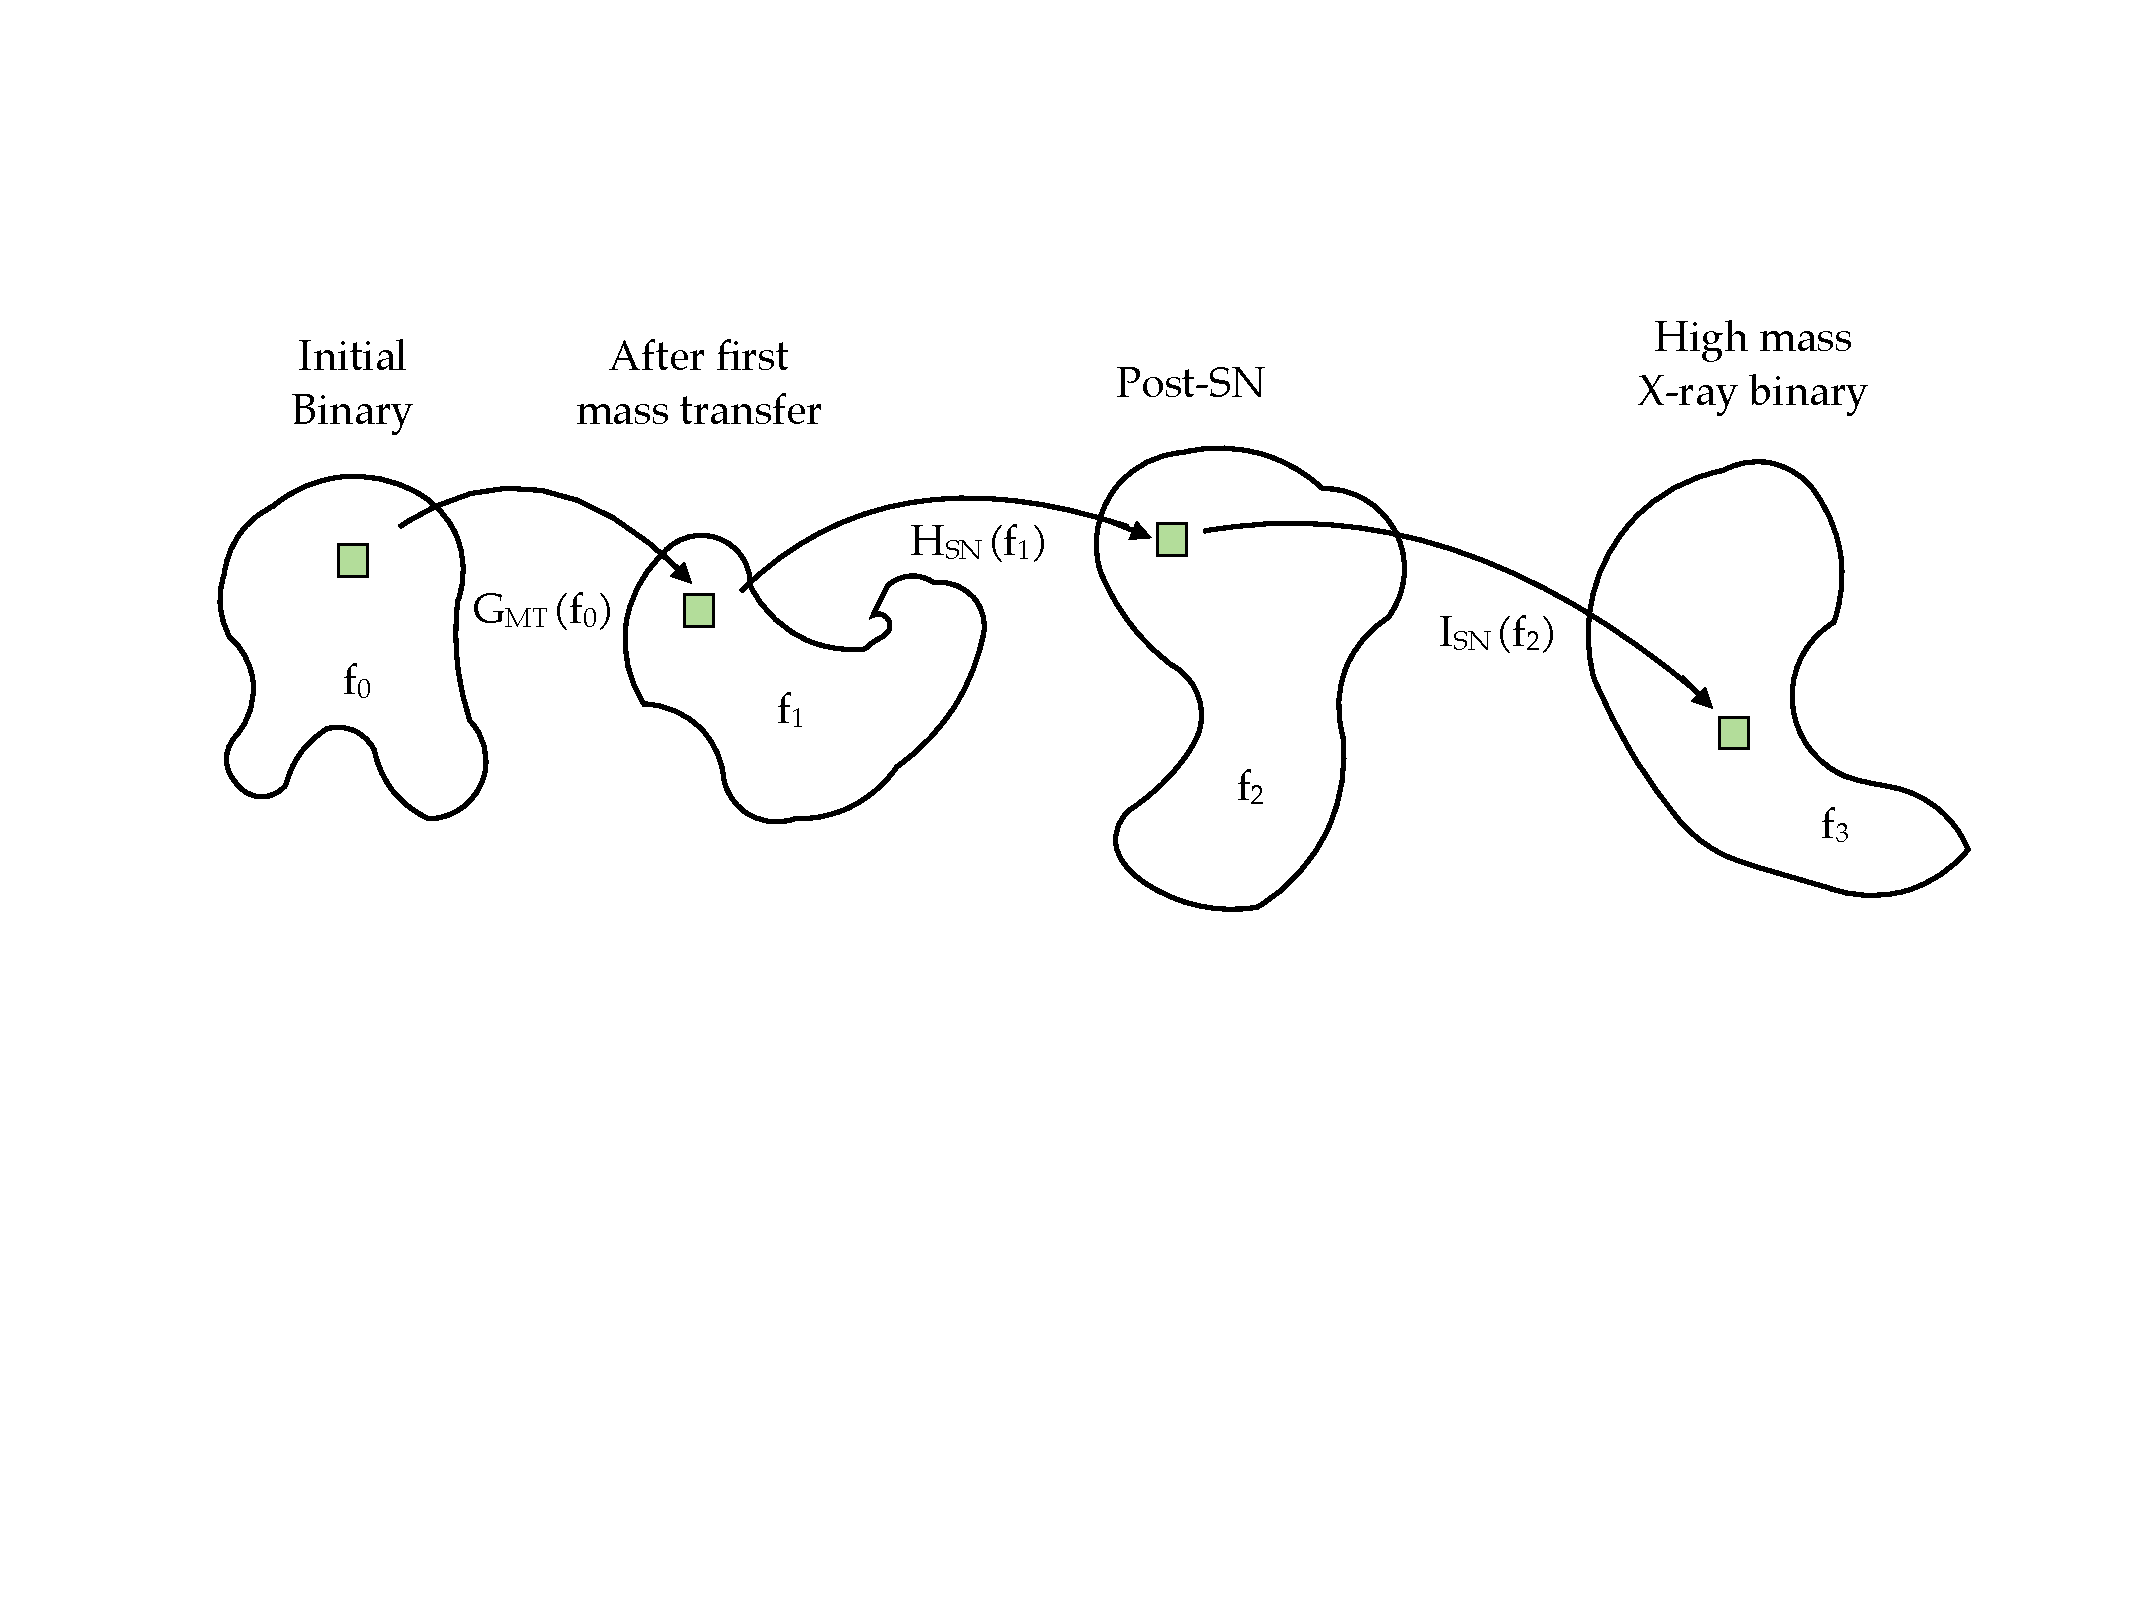
\includegraphics[width=0.95\columnwidth]{Mapping.pdf}
\caption{A mathematical representation of the evolution of a binary from its initial state three separate stages of evolution: the first (stable) mass transfer phase ($G_{\rm MT}$), the primary undergoing core collapse and receiving a natal kick ($H_{\rm SN}$), and the X-ray luminous phase once the second star evolves off the main sequence ($I_{\rm XRB}$). The volume of the three dimensional box around the binary scales with the determinant of the Jacobian matrix for each mapping.}
\label{fig:Mapping}
\end{center}
\end{figure}

Mathematically, these are mappings that can be expressed in a straightforward way:
\begin{eqnarray}
f_1 &=& G_{\rm MT} (f_0) \\
f_2 &=& H_{\rm SN} (f_1) \\
f_3 &=& I_{\rm XRB} (f_2), \\
\end{eqnarray}
which can be combined:
\begin{equation}
f_3 = I_{\rm XRB} \circ H_{\rm SN} \circ G_{\rm MT} ( f_0).
\end{equation}


If we are interesting on an individual system or a small set of binaries, we can opt for a different approach, however.


If, however, a reverse mapping exists (or it can be determined numerically), a different approach can be used. This mapping allows one to determine the initial binary state from the observed system:
\begin{equation}
f_0 = G_{\rm MT}^{-1} \circ H_{\rm SN}^{-1} \circ I_{\rm XRB}^{-1} (f_3) .
\end{equation}
Our model provides the probability of the initial state of the binary, $P(f_0)$. The series of transformations from $f_0$ to $f_3$ each shift the volume of phase space around it, affecting the resulting probability. The probability after each transition is determined by scaling the previous probability by the Jacobian of each transition. Determining the probability of the observed binary is now straightforward:
\begin{eqnarray}
P(f_3) &=& P(f_2)  J_{\rm XRB}  \\
  &=& P(f_1)  J_{\rm SN}  J_{\rm XRB}  \\
  &=& P(f_0)  J_{\rm MT}  J_{\rm SN}  J_{\rm XRB} .
\end{eqnarray}


We choose to adapt and improve upon the Jacobian formalism discussed by Kalogera (1996), Bhadkeamkar \& Ghosh (2012) and others(?). The underlying premise relies upon our ability to map the initial state of a binary through its various stages, until it forms an X-ray luminous object. If this can be done analytically or semi-analytically, such that the first partial derivatives of these mappings can be calculated, then the Jacobians of these mappings can be used to determine how the distribution of binaries evolves without having to randomly generate a population.

If we are interested in determining the probability of any particular binary with some set of observed parameters, such as the set of X-ray binaries in NGC 55, we require both the Jacobians of the three transitions defined above and the reverse mapping. Yet even the most ideal observations of high mass X-ray binaries are unlikely to identify enough parameters to uniquely determine any particular system's prior evolution. To determine the probability of any model producing a binary with observed parameters ($\vec{x}$) we marginalize over latent unobserved parameters ($\vec{y}$):
\begin{equation}
P[f_{\rm obs}(\vec{x})] = \int P[f_3(\vec{x}, \vec{y})] \dd \vec{y}.
\end{equation}
$\vec{y}$ must have enough dimensionality so that the combined $\vec{x}$ and $\vec{y}$ form a complete basis for the binary. This is the basis for the marginalization over $v_k$ and $\theta$ above in Equation \ref{eq:P_marginalized}; $L_x$, $M_2$, and $v_{\rm sys}$ alone do not form a complete basis. In principle, at least, from these five quantities, the initial masses and separation of the binary can be determined.


Below, we discuss each of the three transformations, their reverse mappings, and their Jacobian determinants.


%The reasons for this are many: including complex physics is much easier using Monte Carlo methods, the Jacobian transformation method requires the transformations to be analytic or semi-analytic whereas certain physical processes require numerical integration to accurately calculate, and Monte Carlo methods can easily handle complicated evolutionary channels. 




%Since we are only interested in a small subset of binaries, those that are strong X-ray sources, we can employ the Jacobian transformation method here. The nature of the method is significantly computational cheaper since the region of parameter space explored is, by design, limited to only those binaries we are interested in.
\end{comment}



\end{document}
